% Acoustic Contact Detection Presentation
% Author: Georg Wolnik
% Date: January 31, 2026
%
% NARRATIVE STRUCTURE:
% Act 1 (Slides 1-7): Proof of Concept - Pipeline & Success on Known Data
% Act 2 (Slides 8-12): Discovery - Generalization Challenges (Configuration & Object)
% Act 3 (Slides 13-14): Conclusions and Q&A
% Backup Slides: Additional details for Q&A

\documentclass[aspectratio=169,11pt]{beamer}

% Theme and Colors
\usetheme{Madrid}
\usecolortheme{default}

% Custom colors
\definecolor{successgreen}{RGB}{34, 139, 34}
\definecolor{failurered}{RGB}{220, 20, 60}
\definecolor{highlightblue}{RGB}{0, 102, 204}
\definecolor{neutralgray}{RGB}{128, 128, 128}

\setbeamercolor{frametitle}{bg=highlightblue!20, fg=black}
\setbeamercolor{title}{fg=highlightblue}
\setbeamercolor{block title}{bg=highlightblue, fg=white}
\setbeamercolor{block body}{bg=highlightblue!10}

% Packages
\usepackage{graphicx}
\usepackage{booktabs}
\usepackage{amsmath}
\usepackage{tikz}
\usepackage{fontawesome5}
\usepackage{hyperref}
\usepackage{xcolor}
\usepackage{colortbl}
\usepackage{multirow}
\usepackage{media9}

% Graphics path
\graphicspath{{../presentation_figures/proof_of_concept/}{../presentation_figures/object_generalization/}{../ml_analysis_figures/}{../pattern_a_summary/}{../pattern_b_summary/}{../presentation_animations/}{media/}}

% Title Info
\title[Acoustic Contact Detection]{Geometrical Reconstruction using Acoustic Tactile Sensing}
\subtitle{Can a Robot Hear Whether It Touches Something?}
\author{Georg Wolnik}
\institute{Robotics and Biology Laboratory TU Berlin}
\date{2nd February 2026}

\begin{document}

% ============================================================================
% ACT 1: END-TO-END PIPELINE - PROOF OF CONCEPT (Slides 1-8)
% ============================================================================

% SLIDE 1: TITLE
\begin{frame}[plain]
    \begin{center}
        \vspace{2cm}
        
        {\Huge\color{highlightblue}\textbf{Geometrical Reconstruction using}}\\[0.3cm]
        {\Huge\color{highlightblue}\textbf{Acoustic Tactile Sensing}}
        
        \vspace{0.8cm}
        
        {\Large Can a Robot Hear Whether It Touches Something?}
        
        \vspace{1.5cm}
        
        {\large Georg Wolnik}
        
        \vspace{0.2cm}
        
        {\normalsize Robotics Project - Robotics and Biology Laboratory - TU Berlin}\\[0.2cm]
        {\small 2nd February 2026}
    \end{center}
\end{frame}

% SLIDE 2: MOTIVATION (Problem-Solution-Goal)
\begin{frame}{Motivation}
    \begin{columns}[T]
        % Left column: The Problem
        \begin{column}{0.48\textwidth}
            \begin{block}{\color{highlightblue}The Problem}
                \textbf{Vision isn't always available}
                \begin{itemize}\setlength{\itemsep}{0pt}
                    \item Robot arm/gripper occludes camera view
                    \item Low-light, dusty, or underwater environments
                    \item Need for contact-based perception
                \end{itemize}
            \end{block}
            
            \begin{block}{\color{highlightblue}Why Acoustic Sensing?}
                \begin{itemize}\setlength{\itemsep}{0pt}
                    \item \textbf{Cheap:} Simple contact microphone
                    \item \textbf{Non-invasive:} No complex sensor arrays
                    \item \textbf{Complementary:} Works with vision \& tactile
                \end{itemize}
            \end{block}
        \end{column}
        
        % Right column: Project Goal
        \begin{column}{0.48\textwidth}
            \begin{block}{\color{highlightblue}Project Goal}
                \begin{center}
                    \textit{Can we reconstruct surface geometry from acoustic signals?}
                \end{center}
                \vspace{-0.2cm}
                \begin{itemize}\setlength{\itemsep}{0pt}
                    \item Detect contact events during robot motion
                    \item Classify surface shapes acoustically
                    \item Evaluate generalization capabilities
                \end{itemize}
            \end{block}
        \end{column}
    \end{columns}
\end{frame}

% SLIDE 3: SETUP - THE HARDWARE
\begin{frame}{Setup}
    
    \begin{columns}[T]
        \begin{column}{0.32\textwidth}
            \begin{center}
                \textbf{\color{highlightblue}Full Setup}
                
                \vspace{0.15cm}
                
                \includegraphics[width=\textwidth,height=3.2cm,keepaspectratio]{big_setup.jpeg}
            \end{center}
        \end{column}
        
        \begin{column}{0.32\textwidth}
            \begin{center}
                \textbf{\color{highlightblue}Sensor Mounting}
                
                \vspace{0.15cm}
                
                \includegraphics[width=\textwidth,height=3.2cm,keepaspectratio]{mounting_setup.jpeg}
            \end{center}
        \end{column}
        
        \begin{column}{0.32\textwidth}
            \begin{center}
                \textbf{\color{highlightblue}Close-up}
                
                \vspace{0.15cm}
                
                \includegraphics[width=\textwidth,height=3.2cm,keepaspectratio]{close_setup.jpeg}
            \end{center}
        \end{column}
    \end{columns}
    
    \vspace{0.3cm}
    
    \begin{center}
        \begin{tikzpicture}
            \node[fill=highlightblue!10, rounded corners, inner sep=6pt, text width=0.9\textwidth] {
                \footnotesize\textbf{\color{highlightblue}Why Robot-Mounted Data Collection?}
                \begin{itemize}\setlength{\itemsep}{1pt}\setlength{\parskip}{0pt}
                    \item[\faCheck] \textbf{Controlled variables:} Consistent angle, pressure, and sweep velocity
                    \item[\faCheck] \textbf{Repeatability:} Systematic sweeps for reliable ground truth labels
                    \item[\faCheck] \textbf{Scalability:} Automated collection of large datasets
                    \item[\faCheck] \textbf{Real-world relevance:} Directly applicable to robotic manipulation tasks
                \end{itemize}
            };
        \end{tikzpicture}
    \end{center}
    
\end{frame}


% SLIDE 4: DATA COLLECTION - Objects and Workspaces
\begin{frame}{Data Collection: Objects and Workspaces}
    
    \begin{columns}[T]
        \begin{column}{0.45\textwidth}
            \begin{center}
                \textbf{\color{highlightblue}Test Objects}
                
                \vspace{0.2cm}
                
                \includegraphics[angle=90,width=\textwidth,height=4.5cm,keepaspectratio]{objects.jpeg}
                
                \vspace{0.2cm}
                
                {\footnotesize A: Cutouts | B: Empty | C: Full | D: Big Cutout}
            \end{center}
        \end{column}
        
        \begin{column}{0.52\textwidth}
            \begin{center}
                \textbf{\color{highlightblue}Complete Dataset Overview}
                
                \vspace{0.3cm}
                
                \begin{table}
                    \centering
                    \footnotesize
                    \begin{tabular}{c|cccc}
                        \toprule
                        & \textbf{Obj A} & \textbf{Obj B} & \textbf{Obj C} & \textbf{Obj D} \\
                        & \scriptsize Cutouts & \scriptsize Empty & \scriptsize Full & \scriptsize Big Cut \\
                        \midrule
                        \textbf{WS1} & \cellcolor{successgreen!20}\checkmark & \cellcolor{successgreen!20}\checkmark & \cellcolor{successgreen!20}\checkmark & \\
                        \textbf{WS2} & \cellcolor{successgreen!20}\checkmark & \cellcolor{successgreen!20}\checkmark & \cellcolor{successgreen!20}\checkmark & \\
                        \textbf{WS3} & \cellcolor{successgreen!20}\checkmark & \cellcolor{successgreen!20}\checkmark & \cellcolor{successgreen!20}\checkmark & \\
                        \textbf{WS4} & & & & \cellcolor{failurered!20}\checkmark \\
                        \bottomrule
                    \end{tabular}
                \end{table}
                
                \vspace{0.3cm}
                
                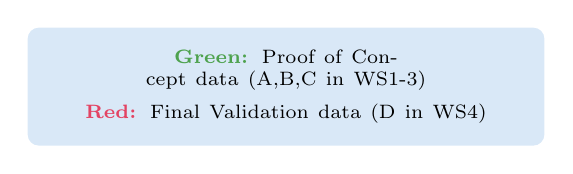
\begin{tikzpicture}
                    \node[fill=highlightblue!15, rounded corners, inner sep=8pt, text width=6cm, align=center] {
                        \scriptsize\textcolor{successgreen!80}{\textbf{Green:}} Proof of Concept data (A,B,C in WS1-3)\\
                        \scriptsize\textcolor{failurered!80}{\textbf{Red:}} Final Validation data (D in WS4)
                    };
                \end{tikzpicture}
            \end{center}
        \end{column}
    \end{columns}
    
\end{frame}

% SLIDE 5: THE GOAL (Single, Focused)
\begin{frame}{Proof of Concept Goal}
    
    \vspace{0.5cm}
    
    \begin{center}
        {\LARGE\color{successgreen}\faQuestion}
        
        \vspace{0.5cm}
        
        {\Huge\textbf{Can we reconstruct geometric shapes}}\\[0.3cm]
        {\Huge\textbf{using binary surface classification?}}
        
        \vspace{0.8cm}
    \end{center}
    
    \begin{columns}[T]
        \begin{column}{0.32\textwidth}
            \begin{block}{\centering Task}
                \centering
                \vspace{0.2cm}
                Binary classification\\[0.2cm]
                \textbf{Contact vs.\ No-Contact}
                \vspace{0.2cm}
            \end{block}
        \end{column}
        
        \begin{column}{0.32\textwidth}
            \begin{block}{\centering Approach}
                \centering
                \vspace{0.2cm}
                Hand-crafted features\\[0.2cm]
                \textbf{80-dim acoustic features}
                \vspace{0.2cm}
            \end{block}
        \end{column}
        
        \begin{column}{0.32\textwidth}
            \begin{block}{\centering Target}
                \centering
                \vspace{0.2cm}
                Geometric reconstruction\\[0.2cm]
                \textbf{on known data}
                \vspace{0.2cm}
            \end{block}
        \end{column}
    \end{columns}
    
    \vspace{0.5cm}
    
    \begin{center}
        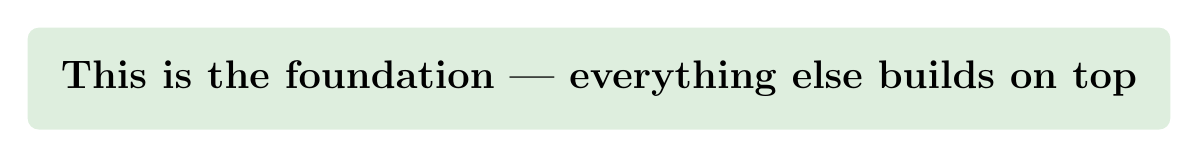
\begin{tikzpicture}
            \node[fill=successgreen!15, rounded corners, inner sep=12pt] {
                \Large\textbf{This is the foundation --- everything else builds on top}
            };
        \end{tikzpicture}
    \end{center}
    
\end{frame}


% SLIDE 6a: METHOD - Core Technical Approach
\begin{frame}{Method: Acoustic Feature Classification}
    
    \begin{center}
        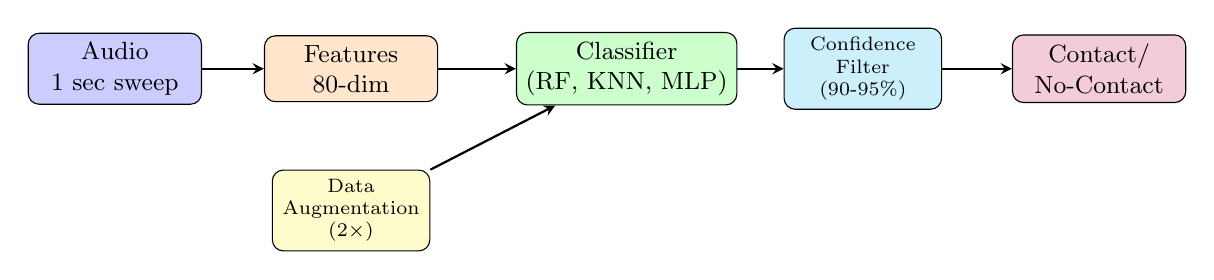
\begin{tikzpicture}[
            box/.style={rectangle, draw, rounded corners, minimum width=2.2cm, minimum height=0.7cm, align=center, font=\small},
            smallbox/.style={rectangle, draw, rounded corners, minimum width=2cm, minimum height=0.5cm, align=center, font=\scriptsize},
            arrow/.style={->, thick, >=stealth}
        ]
            \node[box, fill=blue!20] (audio) at (0,0) {Audio\\1 sec sweep};
            \node[box, fill=orange!20] (features) at (3,0) {Features\\80-dim};
            \node[smallbox, fill=yellow!20] (augment) at (3,-1.8) {Data\\Augmentation\\(2$\times$)};
            \node[box, fill=green!20] (classifier) at (6.5,0) {Classifier\\(RF, KNN, MLP)};
            \node[smallbox, fill=cyan!20] (confidence) at (9.5,0) {Confidence\\Filter\\(90-95\%)};
            \node[box, fill=purple!20] (output) at (12.5,0) {Contact/\\No-Contact};
            
            \draw[arrow] (audio) -- (features);
            \draw[arrow] (features) -- (classifier);
            \draw[arrow] (classifier) -- (confidence);
            \draw[arrow] (confidence) -- (output);
            \draw[arrow] (augment) -- (classifier);
        \end{tikzpicture}
    \end{center}
    
    \begin{columns}[T]
        \begin{column}{0.40\textwidth}
            \begin{block}{80-Dimensional Features}
                \small
                \begin{itemize}\setlength{\itemsep}{0pt}
                    \item \textbf{MFCCs + Deltas} (39): Frequency content
                    \item \textbf{Spectral} (11): Energy distribution
                    \item \textbf{Temporal} (15): Contact dynamics
                    \item \textbf{Impulse Response} (15): Resonance
                \end{itemize}
            \end{block}
        \end{column}
        
        \begin{column}{0.25\textwidth}
            \begin{block}{Data Augmentation}
                \small
                \begin{itemize}\setlength{\itemsep}{0pt}
                    \item Noise injection
                    \item Time shifting
                    \item Pitch variation
                    \item Gain scaling
                    \item Time stretching
                \end{itemize}
            \end{block}
        \end{column}
        
        \begin{column}{0.25\textwidth}
            \begin{alertblock}{Why Hand-Crafted?}
                \small
                \begin{itemize}\setlength{\itemsep}{0pt}
                    \item Hand-crafted: \textcolor{successgreen}{\textbf{73\%}}
                    \item Spectrograms: \textcolor{failurered}{\textbf{59\%}}
                    \item 80 vs 10,240 dims
                \end{itemize}
            \end{alertblock}
        \end{column}
    \end{columns}
    
\end{frame}

% SLIDE 7: MAIN RESULT - Classification Accuracy on Known Data
\begin{frame}{Result: \textcolor{successgreen}{Excellent Classification on Known Data}}
    
    \begin{columns}[T]
        \begin{column}{0.30\textwidth}
            \begin{block}{}
            \centering
            {\LARGE \textcolor{successgreen}{\textbf{$\sim$99\%}}}
  
            {\normalsize Test Accuracy}
            
            {\footnotesize (Known surfaces \& configurations)}
            \end{block}
            
            \begin{block}{Dataset Split}
            \footnotesize
            \centering
            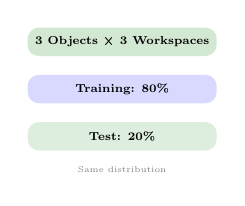
\begin{tikzpicture}[scale=0.6, transform shape]
                % Objects Row
                \node[fill=successgreen!20, rounded corners, minimum width=4cm, minimum height=0.6cm, font=\scriptsize] at (0,2.2) {\textbf{3 Objects × 3 Workspaces}};
                
                % Training Data
                \node[fill=blue!15, rounded corners, minimum width=4cm, minimum height=0.6cm, font=\scriptsize] at (0,1.2) {\textbf{Training: 80\%}};
                
                % Test Data
                \node[fill=successgreen!15, rounded corners, minimum width=4cm, minimum height=0.6cm, font=\scriptsize] at (0,0.2) {\textbf{Test: 20\%}};
                
                % Same distribution note
                \node[font=\tiny, text=gray] at (0,-0.5) {Same distribution};
            \end{tikzpicture}
            \end{block}
        \end{column}
        
        \begin{column}{0.55\textwidth}
            \begin{figure}
            \centering
            \includegraphics[width=\textwidth, height=0.65\textheight, keepaspectratio]{poc_main_result_train_test_only.png}
            \end{figure}
        \end{column}
        \end{columns} 
\end{frame}


% SLIDE 8: VISUAL PROOF - TEST SET (High Accuracy)
\begin{frame}{Reconstruction: Excellent Performance on Test Data}
    
    \begin{columns}[T]
        \begin{column}{0.60\textwidth}
            \begin{figure}
                \centering
                \includegraphics[width=\textwidth, height=0.8\textheight, keepaspectratio]{balanced_workspace_2_squares_cutout_comparison.png}
            \end{figure}
        \end{column}
        
        \begin{column}{0.38\textwidth}
            \begin{block}{What You See}
                \footnotesize
                \begin{itemize}\setlength{\itemsep}{2pt}
                    \item \textbf{Left:} Ground truth surface
                    \item \textbf{Right:} Model reconstruction
                    \item \textcolor{successgreen}{Green} = Contact detected
                    \item \textcolor{failurered}{Red} = No contact
                \end{itemize}
            \end{block}
            
            \vspace{0.3cm}
            
            \begin{alertblock}{TEST Accuracy}
                \centering
                \Large
                \textbf{$\sim$99\%}
                
                \vspace{0.2cm}
                
                \footnotesize
                Model performs excellently on known surfaces\\
                (same distribution as training)
            \end{alertblock}
        \end{column}
    \end{columns}
    
\end{frame}

% ============================================================================
% ACT 2: DISCOVERY - GENERALIZATION CHALLENGES (Slides 9-12)
% ============================================================================

% SLIDE 9: TRANSITION - Now let's test generalization
\begin{frame}{Now: Testing Generalization}
    
    \begin{block}{\centering \textcolor{successgreen}{\faCheckCircle} Proof of Concept Achieved!}
        \centering
        \large
        \textbf{Acoustic contact classification works on known data}\\[0.2cm]
        \footnotesize
        $\sim$100\% test accuracy with excellent reconstruction
    \end{block}
    
    \begin{center}
        {\Large\color{highlightblue}\faSearchPlus}
        
        
        {\LARGE\textbf{But does it generalize?}}\\[0.3cm]
        {\large Two critical questions:}
    \end{center}
    
    
    \begin{columns}[T]
        \begin{column}{0.48\textwidth}
            \begin{block}{\centering What if we test on a \textbf{new workspace}?}
                \centering
                \footnotesize
                Train: WS1+WS3 $\rightarrow$ Test: WS2\\[0.2cm]
                Same objects, \textbf{different robot positions}\\[0.2cm]
                \textcolor{highlightblue}{\faArrowRight{} \textbf{Configuration Generalization}}
            \end{block}
        \end{column}
        
        \begin{column}{0.48\textwidth}
            \begin{block}{\centering What if we test on a \textbf{new object}?}
                \centering
                \footnotesize
                Train: A,B,C $\rightarrow$ Test: D (+ new workspace)\\[0.2cm]
                \textbf{Completely unseen object \& workspace}\\[0.2cm]
                \textcolor{highlightblue}{\faArrowRight{} \textbf{Object Generalization}}
            \end{block}
        \end{column}
    \end{columns}
    
\end{frame}


% SLIDE 10: CONFIGURATION GENERALIZATION - Setup and Results
\begin{frame}{Challenge 1: Configuration Generalization}
    
    \begin{columns}[T]
        \begin{column}{0.45\textwidth}
            \begin{center}
                \textbf{\color{highlightblue}Experimental Setup}
                
                \vspace{0.2cm}
                
                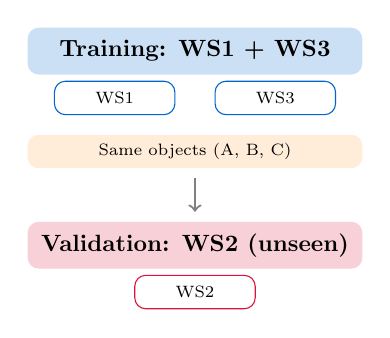
\begin{tikzpicture}[scale=0.85, transform shape]
                    % Training Workspaces
                    \node[fill=highlightblue!20, rounded corners, minimum width=5cm, minimum height=0.7cm] at (0,2.5) {\textbf{Training: WS1 + WS3}};
                    \node[fill=white, rounded corners, draw=highlightblue, minimum width=1.8cm, minimum height=0.5cm, font=\scriptsize] at (-1.2,1.8) {WS1};
                    \node[fill=white, rounded corners, draw=highlightblue, minimum width=1.8cm, minimum height=0.5cm, font=\scriptsize] at (1.2,1.8) {WS3};
                    
                    % Same objects note
                    \node[fill=orange!15, rounded corners, minimum width=5cm, minimum height=0.5cm, font=\scriptsize] at (0,1.0) {Same objects (A, B, C)};
                    
                    % Arrow down
                    \draw[->, thick, gray] (0,0.6) -- (0,0.1);
                    
                    % Validation Workspace
                    \node[fill=failurered!20, rounded corners, minimum width=5cm, minimum height=0.7cm] at (0,-0.4) {\textbf{Validation: WS2 (unseen)}};
                    \node[fill=white, rounded corners, draw=failurered, minimum width=1.8cm, minimum height=0.5cm, font=\scriptsize] at (0,-1.1) {WS2};
                \end{tikzpicture}
                
                \vspace{0.3cm}
                
                {\small \textbf{Same objects, different robot configurations}}
            \end{center}
        \end{column}
        
        \begin{column}{0.52\textwidth}
            \begin{block}{\centering Performance Results}
                \footnotesize
                \centering
                \begin{tabular}{lc}
                    \textbf{Dataset} & \textbf{Accuracy} \\
                    \midrule
                    Training (WS1+WS3) & \textcolor{successgreen}{\textbf{100\%}} \\
                    Test (WS1+WS3, 20\%) & \textcolor{successgreen}{\textbf{$\sim$100\%}} \\
                    \midrule
                    \textbf{Validation (WS2)} & \textcolor{orange}{\textbf{65-75\%}} \\
                \end{tabular}
            \end{block}
            
            \vspace{0.2cm}
            
            \begin{alertblock}{\centering Configuration Entanglement}
                \centering
                {\Large \textcolor{orange}{\textbf{65-75\%}}}\\[0.1cm]
                \footnotesize
                Better than random (50\%), but significant drop\\[0.2cm]
                \textbf{Signal = Contact $\otimes$ Configuration}
            \end{alertblock}
            
            \vspace{0.1cm}
            
            {\footnotesize Model partially learned configuration-specific features. More diverse workspace data likely needed.}
        \end{column}
    \end{columns}
\end{frame}


% SLIDE 11: OBJECT GENERALIZATION - Setup and Results
\begin{frame}{Challenge 2: Object Generalization}
    
    \begin{columns}[T]
        \begin{column}{0.45\textwidth}
            \begin{center}
                \textbf{\color{highlightblue}Object Generalization Setup}
                
                \vspace{0.2cm}
                
                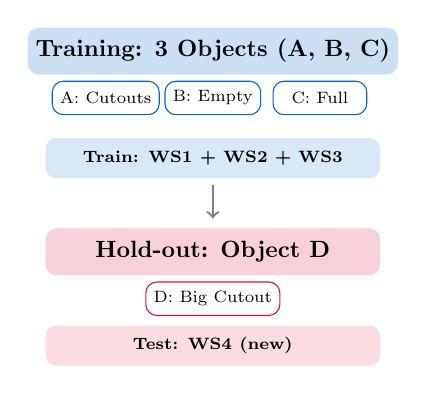
\begin{tikzpicture}[scale=0.85, transform shape]
                    % Objects Row - Training
                    \node[fill=highlightblue!20, rounded corners, minimum width=5cm, minimum height=0.7cm] at (0,2.8) {\textbf{Training: 3 Objects (A, B, C)}};
                    \node[fill=white, rounded corners, draw=highlightblue, minimum width=1.4cm, minimum height=0.5cm, font=\scriptsize] at (-1.6,2.1) {A: Cutouts};
                    \node[fill=white, rounded corners, draw=highlightblue, minimum width=1.4cm, minimum height=0.5cm, font=\scriptsize] at (0,2.1) {B: Empty};
                    \node[fill=white, rounded corners, draw=highlightblue, minimum width=1.4cm, minimum height=0.5cm, font=\scriptsize] at (1.6,2.1) {C: Full};
                    
                    % Training Workspaces
                    \node[fill=highlightblue!15, rounded corners, minimum width=5cm, minimum height=0.6cm, font=\scriptsize] at (0,1.2) {\textbf{Train: WS1 + WS2 + WS3}};
                    
                    % Arrow down
                    \draw[->, thick, gray] (0,0.8) -- (0,0.3);
                    
                    % Hold-out Object
                    \node[fill=failurered!20, rounded corners, minimum width=5cm, minimum height=0.7cm] at (0,-0.2) {\textbf{Hold-out: Object D}};
                    \node[fill=white, rounded corners, draw=failurered, minimum width=2cm, minimum height=0.5cm, font=\scriptsize] at (0,-0.9) {D: Big Cutout};
                    
                    % Hold-out Workspace
                    \node[fill=failurered!15, rounded corners, minimum width=5cm, minimum height=0.6cm, font=\scriptsize] at (0,-1.6) {\textbf{Test: WS4 (new)}};
                \end{tikzpicture}
                
                \vspace{0.3cm}
                
                {\small \textbf{New object + new workspace}\\Complete generalization test}
            \end{center}
        \end{column}
        
        \begin{column}{0.52\textwidth}
            \begin{block}{\centering Performance Results}
                \footnotesize
                \centering
                \begin{tabular}{lc}
                    \textbf{Dataset} & \textbf{Accuracy} \\
                    \midrule
                    Training (A,B,C on WS1-3) & \textcolor{successgreen}{\textbf{100\%}} \\
                    Test (A,B,C on WS1-3) & \textcolor{successgreen}{\textbf{$\sim$100\%}} \\
                    \midrule
                    \textbf{Hold-out (D on WS4)} & \textcolor{failurered}{\textbf{50\%}} \\
                \end{tabular}
            \end{block}
            
            \vspace{0.2cm}
            
            \begin{alertblock}{\centering Critical Discovery}
                \centering
                {\Large \textcolor{failurered}{\textbf{50\% = Random Chance}}}
                
                \vspace{0.2cm}
                \footnotesize
                Model completely fails on unseen object
            \end{alertblock}
        \end{column}
    \end{columns}
    
\end{frame}


% SLIDE 12: ENTANGLEMENT PROBLEM EXPLANATION
\begin{frame}{Understanding the Failure: The Entanglement Problem}
    
    \begin{columns}[T]
        \begin{column}{0.55\textwidth}
            \begin{figure}
                \centering
                \includegraphics[width=\textwidth, height=0.8\textheight, keepaspectratio]{figure7_entanglement_concept.png}
            \end{figure}
        \end{column}
        
        \begin{column}{0.42\textwidth}
            \begin{alertblock}{The Core Problem}
                \centering
                \large
                \textbf{Signal = Contact $\otimes$ Object}
                
                \vspace{0.3cm}
                \footnotesize
                The acoustic signature contains \textbf{BOTH}:\\[0.1cm]
                1. Contact state information\\
                2. Object identity information
            \end{alertblock}
            
            \vspace{0.3cm}
            
            \begin{block}{Physics Explanation}
                \footnotesize
                \begin{itemize}\setlength{\itemsep}{2pt}
                    \item Each object has unique eigenfrequencies
                    \item Material, size, geometry, mass affect acoustic response
                    \item Model learned \textbf{``Object A contact''}\\
                    not \textbf{``contact in general''}
                \end{itemize}
            \end{block}
            
            \vspace{0.3cm}
            
            \begin{block}{Implications}
                \footnotesize
                \begin{itemize}\setlength{\itemsep}{2pt}
                    \item Not a failure --- a \textbf{discovery!}
                    \item Explains 50\% hold-out accuracy
                    \item Future: multi-modal or object-aware models
                \end{itemize}
            \end{block}
        \end{column}
    \end{columns}
    
\end{frame}


% ============================================================================
% ACT 3: CONCLUSIONS (Slides 13-14)
% ============================================================================

% SLIDE 13: CONCLUSIONS
\begin{frame}{Conclusions}
    
    \begin{block}{\textcolor{successgreen}{\faCheckCircle} Main Achievement: Proof of Concept}
        \centering
        \large
        \textbf{``Acoustic-based geometric reconstruction IS POSSIBLE''}\\
        \footnotesize
        (on known data: $\sim$100\% test accuracy, excellent reconstruction)
    \end{block}
    
    \begin{columns}[T]
        \begin{column}{0.48\textwidth}
            \begin{block}{What Works}
                \footnotesize
                \begin{itemize}\setlength{\itemsep}{0pt}
                    \item \textbf{$\sim$99\%} test accuracy\\
                    {\scriptsize (known surfaces \& configurations)}
                    \item Excellent surface reconstruction
                    \item Hand-crafted features outperform\\spectrograms (73\% vs 59\%)
                    \item 128× fewer features, better results
                \end{itemize}
            \end{block}
        \end{column}
        
        \begin{column}{0.48\textwidth}
            \begin{block}{Discovered Limitations}
                \footnotesize
                \begin{itemize}\setlength{\itemsep}{0pt}
                    \item \textbf{Configuration entanglement:}\\
                    65-75\% on unseen workspace\\
                    {\scriptsize Signal = Contact $\otimes$ Configuration}
                    \item \textbf{Object entanglement:}\\
                    50\% on unseen object (random)\\
                    {\scriptsize Signal = Contact $\otimes$ Object}
                \end{itemize}
            \end{block}
        \end{column}
    \end{columns}
    
    
    \begin{block}{Future Directions}
        \footnotesize
        \begin{itemize}\setlength{\itemsep}{0pt}
            \item \textbf{Configuration invariance:} Collect data from many more diverse workspaces/positions
            \item \textbf{Object invariance:} Train on many varied objects to disentangle contact from object identity
        \end{itemize}
    \end{block}
    
\end{frame}

% SLIDE 14: Q&A / THANK YOU
\begin{frame}{Thank You --- Questions?}
    
    \vspace{2cm}
    
    \begin{center}
        {\Huge \textbf{Questions?}}
    \end{center}
    
\end{frame}


% ============================================================================
% BACKUP SLIDES FOR Q&A
% ============================================================================

% BACKUP SLIDE 1: ALL CLASSIFIERS COMPARISON
\begin{frame}[noframenumbering]{Backup: All Classifiers Comparison}
    
    \begin{columns}[T]
        \begin{column}{0.55\textwidth}
            \begin{figure}
                \centering
                \includegraphics[width=\textwidth, height=0.75\textheight, keepaspectratio]{../results_v11/discriminationanalysis/validation_results/classifier_performance.png}
            \end{figure}
        \end{column}
        
        \begin{column}{0.42\textwidth}
            \begin{block}{Top Classifiers (Validation)}
                \footnotesize
                \begin{tabular}{lr}
                    \textbf{Classifier} & \textbf{Val Acc.} \\
                    \midrule
                    MLP (Medium-HighReg) & \textbf{72.0\%} \\
                    GPU-MLP (Tuned-HighReg) & 71.9\% \\
                    Ensemble (Top3-MLP) & 71.3\% \\
                    MLP (Large) & 68.9\% \\
                    GPU-MLP (Tuned) & 68.6\% \\
                    Gradient Boosting & 65.1\% \\
                    Random Forest & 60.1\% \\
                \end{tabular}
            \end{block}
            
            \vspace{0.2cm}
            
            \begin{alertblock}{Key Finding}
                \footnotesize
                \centering
                MLPs with regularization\\
                outperform tree-based methods\\
                on validation data
            \end{alertblock}
        \end{column}
    \end{columns}
    
\end{frame}

% BACKUP SLIDE 2: FEATURE LIST (80 dimensions)
\begin{frame}[noframenumbering]{Backup: 80-Dimensional Feature Set}
    
    \begin{columns}[T]
        \begin{column}{0.48\textwidth}
            \begin{block}{MFCCs + Deltas (39 dims)}
                \footnotesize
                \begin{itemize}\setlength{\itemsep}{1pt}
                    \item 13 MFCC coefficients
                    \item 13 MFCC delta (velocity)
                    \item 13 MFCC delta-delta (acceleration)
                \end{itemize}
            \end{block}
            
            \vspace{0.2cm}
            
            \begin{block}{Spectral Features (11 dims)}
                \footnotesize
                \begin{itemize}\setlength{\itemsep}{1pt}
                    \item Spectral centroid
                    \item Spectral bandwidth
                    \item Spectral rolloff
                    \item Spectral flatness
                    \item Spectral contrast (7 bands)
                \end{itemize}
            \end{block}
        \end{column}
        
        \begin{column}{0.48\textwidth}
            \begin{block}{Temporal Features (15 dims)}
                \footnotesize
                \begin{itemize}\setlength{\itemsep}{1pt}
                    \item Zero-crossing rate
                    \item RMS energy
                    \item Mean, std, skewness, kurtosis
                    \item Onset strength
                    \item Tempo estimation
                \end{itemize}
            \end{block}
            
            \vspace{0.2cm}
            
            \begin{block}{Impulse Response (15 dims)}
                \footnotesize
                \begin{itemize}\setlength{\itemsep}{1pt}
                    \item Transfer function peaks
                    \item Decay characteristics
                    \item Resonance frequencies
                    \item Damping coefficients
                \end{itemize}
            \end{block}
            
            \vspace{0.2cm}
            
            \begin{alertblock}{Total: 80 Features}
                \footnotesize
                \centering
                39 + 11 + 15 + 15 = 80 dimensions\\
                vs.\ spectrograms: 10,240 dimensions
            \end{alertblock}
        \end{column}
    \end{columns}
    
\end{frame}

% BACKUP SLIDE 3: OBJECT AND WORKSPACE DETAILS
\begin{frame}[noframenumbering]{Backup: Object and Workspace Details}
    
    \begin{columns}[T]
        \begin{column}{0.48\textwidth}
            \begin{block}{Training Objects (A, B, C)}
                \footnotesize
                \begin{itemize}\setlength{\itemsep}{2pt}
                    \item \textbf{Object A:} Cutouts\\
                    {\scriptsize Wooden board with geometric cutouts}
                    \item \textbf{Object B:} Empty\\
                    {\scriptsize Plain wooden surface}
                    \item \textbf{Object C:} Full\\
                    {\scriptsize Wooden board with filled shapes}
                \end{itemize}
            \end{block}
            
            \vspace{0.2cm}
            
            \begin{block}{Hold-out Object (D)}
                \footnotesize
                \begin{itemize}\setlength{\itemsep}{2pt}
                    \item \textbf{Object D:} Big cutout\\
                    {\scriptsize Larger wooden board with single large cutout}
                    \item Tested in WS4 only
                    \item Never seen during training
                \end{itemize}
            \end{block}
        \end{column}
        
        \begin{column}{0.48\textwidth}
            \begin{block}{Configuration Generalization Test}
                \footnotesize
                \begin{itemize}\setlength{\itemsep}{2pt}
                    \item \textbf{Train:} WS1, WS3 (Objects A,B,C)
                    \item \textbf{Validate:} WS2 (Objects A,B,C)
                    \item Tests \textbf{configuration generalization}
                    \item Result: \textcolor{orange}{\textbf{65-75\%}} (partial)
                \end{itemize}
            \end{block}
            
            \vspace{0.2cm}
            
            \begin{block}{Object Generalization Test}
                \footnotesize
                \begin{itemize}\setlength{\itemsep}{2pt}
                    \item \textbf{Train:} WS1,2,3 (Objects A,B,C)
                    \item \textbf{Hold-out:} WS4 (Object D)
                    \item Tests \textbf{object generalization}
                    \item Result: \textcolor{failurered}{\textbf{50\%}} (random)
                \end{itemize}
            \end{block}
        \end{column}
    \end{columns}
    
\end{frame}

% BACKUP SLIDE 4: ENTANGLEMENT PROBLEM DETAIL
\begin{frame}[noframenumbering]{Backup: The Entanglement Problem Explained}
    
    \begin{columns}[T]
        \begin{column}{0.55\textwidth}
            \begin{figure}
                \centering
                \includegraphics[width=\textwidth, height=0.6\textheight, keepaspectratio]{figure7_entanglement_concept.png}
            \end{figure}
        \end{column}
        
        \begin{column}{0.42\textwidth}
            \begin{alertblock}{Two Entanglement Problems}
                \centering
                \footnotesize
                \textbf{1. Signal = Contact $\otimes$ Configuration}\\
                Robot pose affects acoustic response\\[0.2cm]
                \textbf{2. Signal = Contact $\otimes$ Object}\\
                Object identity entangled with contact
            \end{alertblock}
            
            \vspace{0.2cm}
            
            \begin{block}{Physics Explanation}
                \footnotesize
                \begin{itemize}\setlength{\itemsep}{1pt}
                    \item Robot pose affects wave propagation
                    \item Each object has unique eigenfrequencies
                    \item Material, size, geometry affect response
                \end{itemize}
            \end{block}
            
            \vspace{0.2cm}
            
            \begin{block}{Implications}
                \footnotesize
                \begin{itemize}\setlength{\itemsep}{1pt}
                    \item Not failures --- \textbf{discoveries}
                    \item Configuration: 65-75\% (partial)
                    \item Object: 50\% (random chance)
                    \item Both need more diverse training data
                \end{itemize}
            \end{block}
        \end{column}
    \end{columns}
    
\end{frame}

% BACKUP SLIDE 5: HAND-CRAFTED vs SPECTROGRAMS COMPARISON
\begin{frame}[noframenumbering]{Backup: Hand-Crafted Features vs Spectrograms}
    
    \begin{columns}[T]
        \begin{column}{0.55\textwidth}
            \begin{figure}
                \includegraphics[width=\textwidth]{handcrafted_vs_spectrogram_comparison.png}
            \end{figure}
        \end{column}
        
        \begin{column}{0.42\textwidth}
            \begin{block}{Key Results}
                \small
                \textbf{Validation Accuracy (WS2+3→WS1):}
                \begin{itemize}\setlength{\itemsep}{2pt}
                    \item \textcolor{successgreen}{\textbf{Hand-Crafted: 73.4\%}}
                    \item \textcolor{failurered}{Spectrograms: 59.3\%}
                    \item \textbf{+14.1\% improvement!}
                \end{itemize}
            \end{block}
            
            \vspace{0.2cm}
            
            \begin{alertblock}{Why Hand-Crafted Wins}
                \footnotesize
                \begin{itemize}\setlength{\itemsep}{2pt}
                    \item \textbf{128× fewer features} (80 vs 10,240)
                    \item \textbf{Less overfitting} with limited data
                    \item \textbf{More interpretable} features
                    \item \textbf{Faster inference} (<1ms)
                    \item \textbf{Better generalization}
                \end{itemize}
            \end{alertblock}
            
            \vspace{0.2cm}
            
            \begin{block}{Conclusion}
                \footnotesize
                \centering
                \textbf{``Less is more''}\\[0.1cm]
                80 well-designed features\\
                outperform 10,240 raw features!
            \end{block}
        \end{column}
    \end{columns}
    
\end{frame}

\end{document}